\documentclass[conference,a4paper]{IEEEtran}
\IEEEoverridecommandlockouts
\usepackage{cite}
\usepackage{amsmath,amssymb,amsfonts}
\usepackage{graphicx}
\usepackage{booktabs}
\usepackage{multirow}
\usepackage{array}
\usepackage{enumitem}
\usepackage{float}
\usepackage{textcomp}
\usepackage{hyperref}
\usepackage{xcolor}
\usepackage{xurl}
\usepackage{balance}
\hypersetup{colorlinks=true, linkcolor=blue, citecolor=blue, urlcolor=cyan}
\renewcommand{\IEEEkeywordsname}{Keywords}
\begin{document}


\title{
\makebox[\textwidth][l]{%
\parbox{\textwidth}{%
\fontsize{9}{11}\selectfont
2026 IEEE 3rd International Student Conference on Digital Generation\\
21--23 October, 2026, Astana, Kazakhstan
}}
\\[1.2em]
\fontsize{20}{24}\selectfont
Physics-Informed Neural Networks for Predicting Caspian Sea Level Variations: A Comparative Study of Water-Balance, Budyko, and Energy-Balance Constraints
}
\author{
\IEEEauthorblockN{
Bekzat Ashirbek,
Arlan Mirseiit,
Amir Nurseit,
Anar Rakhimzhanova
}
\IEEEauthorblockA{
School of AI and Data Science\\
Astana IT University\\
Astana, Kazakhstan\\
Emails: \{bekzatashirbek2, arionzo2005, a2n19a2n\}@gmail.com,
a.rakhymzhanova@astanait.edu.kz\\
ORCID (Ashirbek): 0009-0007-9393-2446\\
ORCID (Mirseiit): 0009-0001-4851-5578,
(Nurseit): 0009-0006-1380-7278\\
ORCID (Rakhimzhanova): 0000-0003-4646-0603
}
}

\maketitle



\begin{abstract}
We develop three Physics-Informed Neural Network (PINN) formulations, based on water balance, the Budyko framework, and the Priestley Taylor energy balance, for predicting Caspian Sea level variations using an identical CNN-LSTM backbone. Across 60 models trained with five random seeds, PINN-3 achieves the highest coefficient of determination, with a mean value of 0.6939 and a standard deviation of 0.0032, while demonstrating exceptional stability. Physics constraints reduce seed-to-seed variation in the coefficient of determination by factors ranging from 2 to 17 and enable positive predictive performance at 10-day resolution where the unconstrained baseline fails. Simple persistence and climatology baselines achieve coefficient of determination values of 0.017 and 0.0, respectively, confirming the added value of the neural models. We contribute a reproducible data-integration pipeline and an empirical framework for evaluating physics constraints in closed-basin modeling.
\end{abstract}

\begin{IEEEkeywords}
Caspian Sea, PINN, CNN--LSTM, water balance, Budyko, Priestley--Taylor, ERA5
\end{IEEEkeywords}

\section{Introduction}

The Caspian Sea, the world's largest inland water body (${\sim}371{,}000$~km$^2$), has declined approximately 1.5~m between 1996 and 2021~\cite{samant2023climate}. CMIP6 projections indicate continued decline, with significant implications for coastal infrastructure and ecosystems. The mean $\Delta H$ during the 2018--2026 test period ($-0.031$~m/month) represents an approximately eightfold acceleration relative to 1993--2014 ($-0.004$~m/month).

Predicting these changes is challenging: purely data-driven methods may violate physical conservation laws, while traditional physical models are limited by uncertain inputs~\cite{saraceni2025water}. Physics-Informed Neural Networks (PINNs)~\cite{raissi2019physics} embed physical constraints into neural network training, minimizing both data misfit and governing equation residuals. The approach has been extended to sea-surface-height prediction~\cite{huang2025physics} and hydrological mass-consistency~\cite{bhasme2021physics}.

Within hydrology, the Budyko framework constrains catchment-scale water partitioning~\cite{cheng2025global}. Liu et al.~\cite{liu2025timevarying} showed Budyko parameters evolve over time, motivating time-varying constraints. For the Caspian Sea, Samant and Prange~\cite{samant2023climate} produced CMIP6 projections; Eftekhari et al.~\cite{eftekhari2024evaluation} evaluated ML methods using GRACE data; Saraceni et al.~\cite{saraceni2025water} developed ERA5-Land water balance procedures. Across these studies, consistent patterns emerge: water-level change is fundamentally a flux partitioning problem; constraints are useful only when matched to dominant processes and not imposed too strongly~\cite{huang2025physics,cuomo2022pinn}; sparse data do not preclude physics-guided modeling~\cite{podina2023universal}; and hydrological parameters should not be assumed constant~\cite{liu2025timevarying}.

Despite this progress, several gaps persist: no PINN exists for the Caspian Sea; no framework links catchment runoff, basin water balance, and whole-sea level; systematic comparison of multiple constraints against an identical backbone is absent; and the question of whether physics constraints improve predictive skill or merely add interpretability remains open.

This work addresses these gaps through: (1) a reproducible multi-source data-integration pipeline combining ERA5, ERA5-Land, GLDAS, DAHITI, and GloFAS data over 1993--2026; and (2) a comprehensive empirical comparison of three PINN formulations against an unconstrained baseline, supported by 60 trained models across five seeds, $\lambda_{\text{phys}}$ sensitivity analysis, walk-forward cross-validation, Monte Carlo dropout, ablation studies, and a hybrid architecture.

\section{Data and Methods}

\subsection{Data Sources and Preprocessing}

The study domain covers a regridded $110 \times 90$ grid at $0.25^\circ$ resolution over the Caspian Sea region. Five products were integrated: ERA5~\cite{hersbach2020era5}, ERA5-Land~\cite{munoz2021eraland}, GLDAS Noah~\cite{rodell2004gldas}, DAHITI altimetry (ID~39)~\cite{schwatke2015dahiti}, and GloFAS Volga discharge~\cite{grimaldi2022glofas}. ERA5 data were extracted via CDS API on a month-by-month basis. Derived variables included VPD (FAO-56~\cite{allen1998fao}) and basin aridity. A land--water mask excluded mixed-boundary grid cells before lake-scale averaging.

Data were split chronologically: training (1993--2014, 67\%), validation (2015--2017, 9\%), testing (2018--2026, 24\%). The test set was never used for hyperparameter selection; all tuning used validation-set metrics only. Monthly (396 steps), 10-day (1,193 steps), and daily (12,103 steps) resolutions were produced. Input consists of 13 gridded channels (Table~\ref{tab:input}) with a 6-step look-back window.

\begin{table}[htbp]
\centering
\caption{Input variables (all $110{\times}90$, $0.25^\circ$ grid).}
\label{tab:input}
\footnotesize
\setlength{\tabcolsep}{3pt}
\begin{tabular}{c>{\raggedright\arraybackslash}p{3.8cm}>{\raggedright\arraybackslash}p{2.6cm}}
\toprule
\# & Variable & Units \\
\midrule
1--6 & Precip., temp., solar/thermal rad., pressure, evap. & m, K, J/m$^2$, Pa, m \\
7--9 & Dewpoint, \textit{u}-wind, \textit{v}-wind & K, m/s \\
10--12 & Surface/sub-surface runoff, SWE & m \\
13 & Volga discharge (broadcast) & m$^3$/s \\
\bottomrule
\end{tabular}
\end{table}

\subsection{CNN--LSTM Backbone}

All models share an identical CNN--LSTM backbone (${\sim}339$K parameters). The spatial encoder uses two Conv2d blocks (in$\to$32$\to$64 channels, AdaptiveAvgPool to $4{\times}4$, producing 1024 features/time step). A two-layer LSTM (hidden=64, dropout=0.5) processes the 6-step sequence; only the final hidden state is retained. The regression head is Linear(64$\to$64)$\to$Activation$\to$Dropout(0.5)$\to$Linear(64$\to D_{\text{out}}$). The backbone structure (layer count, dimensions, connectivity) is identical across all models. Activation functions differ (ReLU: baseline, PINN-1; SiLU: PINN-2, PINN-3), chosen per model based on preliminary validation. While this introduces a potential confound (discussed in \S~\ref{sec:limitations}), the shared spatial and temporal architecture isolates the first-order effect of physics formulations. The shared backbone architecture is shown in Fig.~\ref{fig:architecture}.

\begin{figure}[htbp]
    \centering
    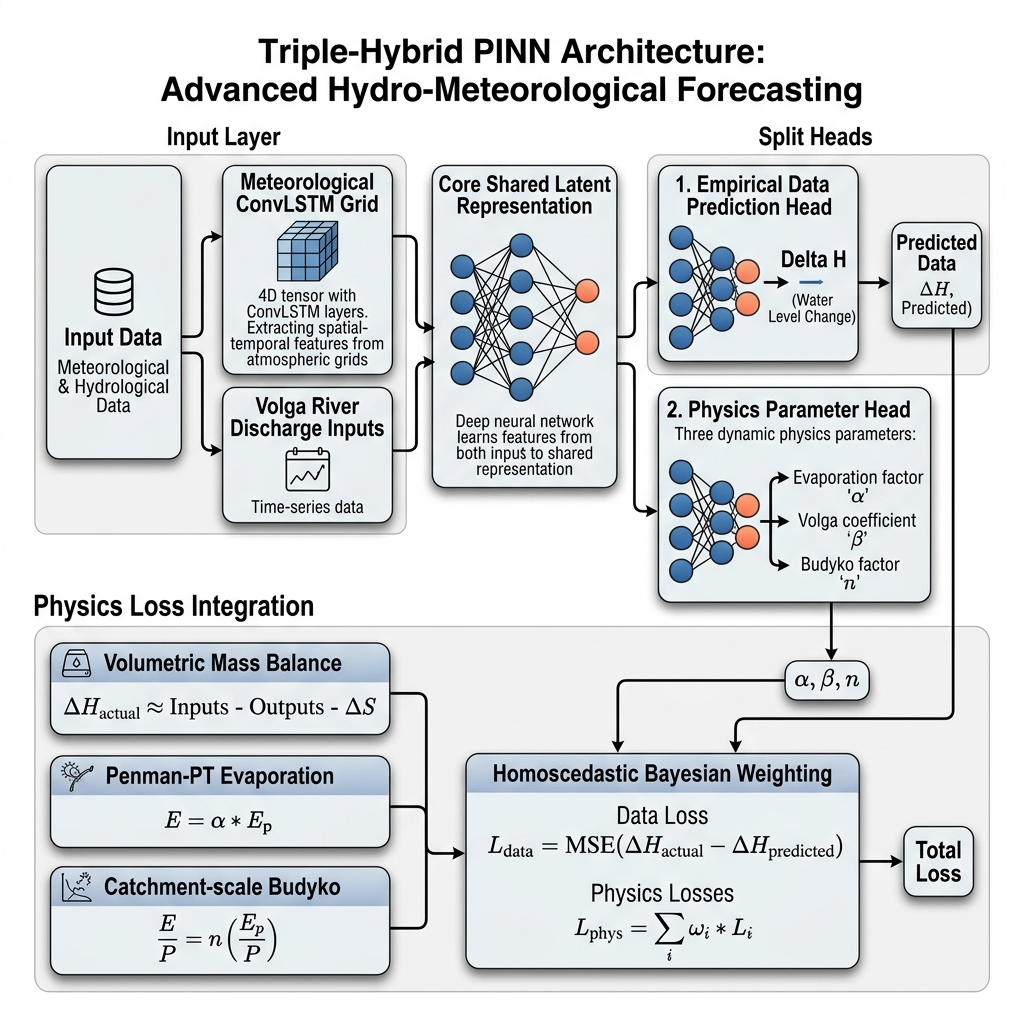
\includegraphics[width=\columnwidth]{../../figures/review_figures/fig3_1_triple_hybrid_architecture.png}
    \caption{CNN--LSTM backbone shared by all models.}
    \label{fig:architecture}
\end{figure}

\subsection{Training Configuration}

Table~\ref{tab:training} summarizes hyperparameters. Each model's hyperparameters were tuned independently, as different physics constraints require different optimization strategies. All models use AdamW (weight\_decay=0.05), CosineAnnealingLR, sequence length~6, gradient clipping~1.0, and patience~50.

\textbf{PINN-1 $\lambda_{\text{phys}}$ note.} The main multi-seed PINN-1 was run at $\lambda_{\text{phys}}{=}100$ (initial configuration). Subsequent sensitivity analysis identified $\lambda_{\text{phys}}{=}1.0$ as optimal (single-seed $R^2{=}0.6211$). Multi-seed retraining at $\lambda_{\text{phys}}{=}1.0$ produced $R^2{=}0.6268\pm0.0230$ (Table~\ref{tab:ranking}). PINN-1's original multi-seed results represent a suboptimal configuration.

\begin{table}[htbp]
\centering
\caption{Training configuration (monthly).}
\label{tab:training}
\begin{tabular}{lcccc}
\toprule
\textbf{Model} & \textbf{Epochs} & \textbf{Batch} & \textbf{LR} & $\lambda_{\text{phys}}$ \\
\midrule
Baseline & 600 & 16 & $1{\times}10^{-4}$ & --- \\
PINN-1   & 600 & 16 & $1{\times}10^{-4}$ & 100 \\
PINN-2   & 300 & 16 & $3{\times}10^{-4}$ & Learned\textsuperscript{a} \\
PINN-3   & 300 & 16 & $3{\times}10^{-4}$ & 1.0 \\
\bottomrule
\multicolumn{5}{>{\raggedright\arraybackslash}p{\columnwidth}}{\textsuperscript{a}Learned homoscedastic uncertainty weighting~\cite{kendall2017uncertainty}: $\lambda_{\text{data}}=e^{-\log\sigma^2_{\text{data}}}$, $\lambda_{\text{phys}}=e^{-\log\sigma^2_{\text{phys}}}$, with $\sigma$ learned during training.}\\
\end{tabular}
\end{table}

\subsection{PINN Formulations}

All PINNs minimize $\mathcal{L}_{\text{total}} = \mathcal{L}_{\text{data}} + \lambda_{\text{phys}}\mathcal{L}_{\text{phys}}$, where $\mathcal{L}_{\text{phys}} = \text{MSE}(\Delta h_{\text{pred}}, \Delta h_{\text{phys}})$. The CNN--LSTM backbone predicts $\Delta h_{\text{pred}}$ plus model-specific physics parameters (softplus-constrained to physically valid ranges).

\textbf{PINN-1 (Water Balance):}
\begin{equation}
\begin{split}
\Delta h_{\text{phys}} &= (P_{\text{lake}} - \alpha_E E_{\text{lake}}) \\
&\quad + \beta_{\text{volga}} \frac{Q_{\text{volga}}\Delta t}{A_{\text{lake}}} \\
&\quad + \gamma_{\text{other}} \max(0, P_{\text{basin}} - PET_{\text{basin}})
\end{split}
\label{eq:pinn1}
\end{equation}
with $A_{\text{lake}}{=}3.71{\times}10^{11}$~m$^2$. Additional prior and mean-bias penalties are applied.

\textbf{PINN-2 (Budyko):} Uses the Choudhury-Yang parameterization~\cite{choudhury1999evaluation,yang2008new} with time-varying exponent $n_t{\geq}1.0$:
\begin{align}
\phi_t &= \frac{PET_{\text{basin},t}}{P_{\text{basin},t} + \varepsilon} \label{eq:aridity} \\
ET_{\text{budyko},t} &= \left[ \frac{\phi_t}{(1 + \phi_t^{n_t})^{1/n_t}} \right] P_{\text{basin},t} \label{eq:budyko} \\
\Delta h_{\text{phys},t} &= (P_{\text{basin},t} - ET_{\text{budyko},t}) \cdot \text{scale}_t \nonumber\\
&\quad + (P_{\text{lake},t} - E_{\text{lake},t}) \label{eq:pinn2}
\end{align}
While originally developed for annual scales, the time-varying $n_t$ is specifically designed to capture seasonal dynamics. Sub-annual Budyko applications have shown utility when parameters are allowed to vary~\cite{liu2025timevarying}. Learned homoscedastic uncertainty weighting~\cite{kendall2017uncertainty} balances data and physics losses. The PINN-2 River variant (see Appendix) adds explicit Volga discharge scaling.

\textbf{PINN-3 (Priestley--Taylor):} Evaporation is parameterized via psychrometric quantities (FAO-56~\cite{allen1998fao}) with learnable $\alpha_{\text{PT},t}{\geq}1.0$~\cite{priestley1972taylor} and $C_{\text{wind},t}{>}0$:
\begin{align}
e_s(T_t) &= 0.6108 \exp\!\left(\frac{17.27\,T_t}{T_t+237.3}\right) \\
e_a(T_{d,t}) &= 0.6108 \exp\!\left(\frac{17.27\,T_{d,t}}{T_{d,t}+237.3}\right) \nonumber\\
\text{VPD}_t &= \max(0,\, e_s - e_a) \\
\Delta_t &= \frac{4098\,e_s}{(T_t+237.3)^2} \\
\gamma_t &= 0.665\times10^{-3} P_t \label{eq:psychro}
\end{align}
\begin{equation}
\begin{split}
E_{\text{lake},t}^{\text{phys}} &= \alpha_{\text{PT},t} \frac{\Delta_t}{\Delta_t + \gamma_t} R^{\text{eq}}_{n,t} \\
&\quad + C_{\text{wind},t} \frac{\gamma_t}{\Delta_t + \gamma_t} (1 + 0.536U_t)\,\text{VPD}_t \label{eq:pinn3_evap}
\end{split}
\end{equation}

\textbf{Hybrid PINN} (see Appendix) combines all three constraints. The Hybrid and ablation experiments were evaluated as single-seed runs due to computational constraints.

\subsection{Experimental Design}

Two-stage evaluation: Stage~1 used PINN-2 to screen temporal resolutions (daily excluded). Stage~2 comprised: (1) Multi-seed training across five seeds (42, 123, 2024, 7, 999) at all three resolutions (60 models); (2) $\lambda_{\text{phys}}$ sensitivity ($\lambda{\in}\{0.1,0.5,1.0,5.0\}$); (3) MC dropout (100 forward passes); (4) Ablation (no residual, dynamic lake area, Hybrid); (5) Walk-forward CV (three expanding-window folds); (6) Thermodynamic walk-forward. All primary metrics use $\Delta H$ (month-to-month change), a more conservative indicator than absolute level $H$.

The effective sample count is approximately 390 sequences (6-month sliding windows from 396 monthly steps). Overfitting is mitigated by early stopping and the chronological split; training/validation loss curves (Fig.~\ref{fig:supplementary}) confirm no severe overfitting.

\section{Results}

\subsection{Temporal Screening and Simple Baselines}

PINN-2 screening (Table~\ref{tab:screening}) established monthly as the primary scale. Daily resolution was excluded ($R^2{=}{-}1.2358$). Simple baselines computed from test data confirm all neural models add substantial value: persistence ($\Delta H_t{=}\Delta H_{t-1}$) achieves $\text{RMSE}{=}0.0874$, $R^2{=}0.017$; climatology (training mean $\Delta H$) achieves $\text{RMSE}{=}0.0878$, $R^2{=}0.0$.

\begin{table}[htbp]
\centering
\caption{Temporal screening and simple baselines.}
\label{tab:screening}
\begin{tabular}{lccc}
\toprule
\textbf{Model} & \textbf{RMSE (m)} & \textbf{$R^2$} & \textbf{Status} \\
\midrule
PINN-2 daily      & 0.0147 & $-$1.2358 & Excluded \\
PINN-2 10-day     & 0.0502 & 0.0126    & Suppl. \\
PINN-2 monthly    & 0.0555 & 0.6007    & Primary \\
Persistence       & 0.0874 & 0.017     & Baseline \\
Climatology       & 0.0878 & 0.000     & Baseline \\
\bottomrule
\end{tabular}
\end{table}

\subsection{Monthly Multi-Seed Results}

Table~\ref{tab:multiseed} reports the primary five-seed monthly $\Delta H$ results.

\begin{table}[htbp]
\centering
\caption{Monthly multi-seed $\Delta H$ results (mean $\pm$ std, $n{=}5$).}
\label{tab:multiseed}
\begin{tabular}{lccc}
\toprule
\textbf{Model} & \textbf{RMSE (m)} & \textbf{Corr.} & \textbf{$R^2$} \\
\midrule
Persistence    & 0.0874 & ---   & 0.017 \\
Climatology    & 0.0878 & ---   & 0.000 \\
Baseline       & $0.0568{\pm}0.0038$ & $0.7844{\pm}0.0240$ & $0.5803{\pm}0.0556$ \\
PINN-1         & $0.0605{\pm}0.0013$ & $0.8211{\pm}0.0080$ & $0.5252{\pm}0.0205$ \\
PINN-2         & $0.0572{\pm}0.0018$ & $0.7969{\pm}0.0192$ & $0.5756{\pm}0.0259$ \\
PINN-3         & $0.0486{\pm}0.0003$ & $0.8341{\pm}0.0016$ & $0.6939{\pm}0.0032$ \\
\bottomrule
\end{tabular}
\end{table}

PINN-3 achieves the best performance with exceptional stability ($R^2$ std~=~0.0032). Physics constraints reduce seed sensitivity substantially: PINN-3~$\pm0.0032$ vs.~baseline~$\pm0.0556$. The Diebold-Mariano test~\cite{diebold1995comparing}, applied to baseline seed pairs, confirms significant inter-seed variability (DM~=~$-2.4$ to $+2.7$, $p{<}0.01$ for 7/10 pairs), quantitatively validating our claim that single-seed baseline results are unreliable.

At 10-day resolution (Appendix), only physics-informed models achieve positive $R^2$ (PINN-1: $0.0827{\pm}0.0302$, PINN-2: $0.1025{\pm}0.0241$), while the baseline remains negative ($-0.1722{\pm}0.0555$). Fig.~\ref{fig:pinn3_monthly} shows the PINN-3 reconstruction over the test period.

\begin{figure}[htbp]
    \centering
    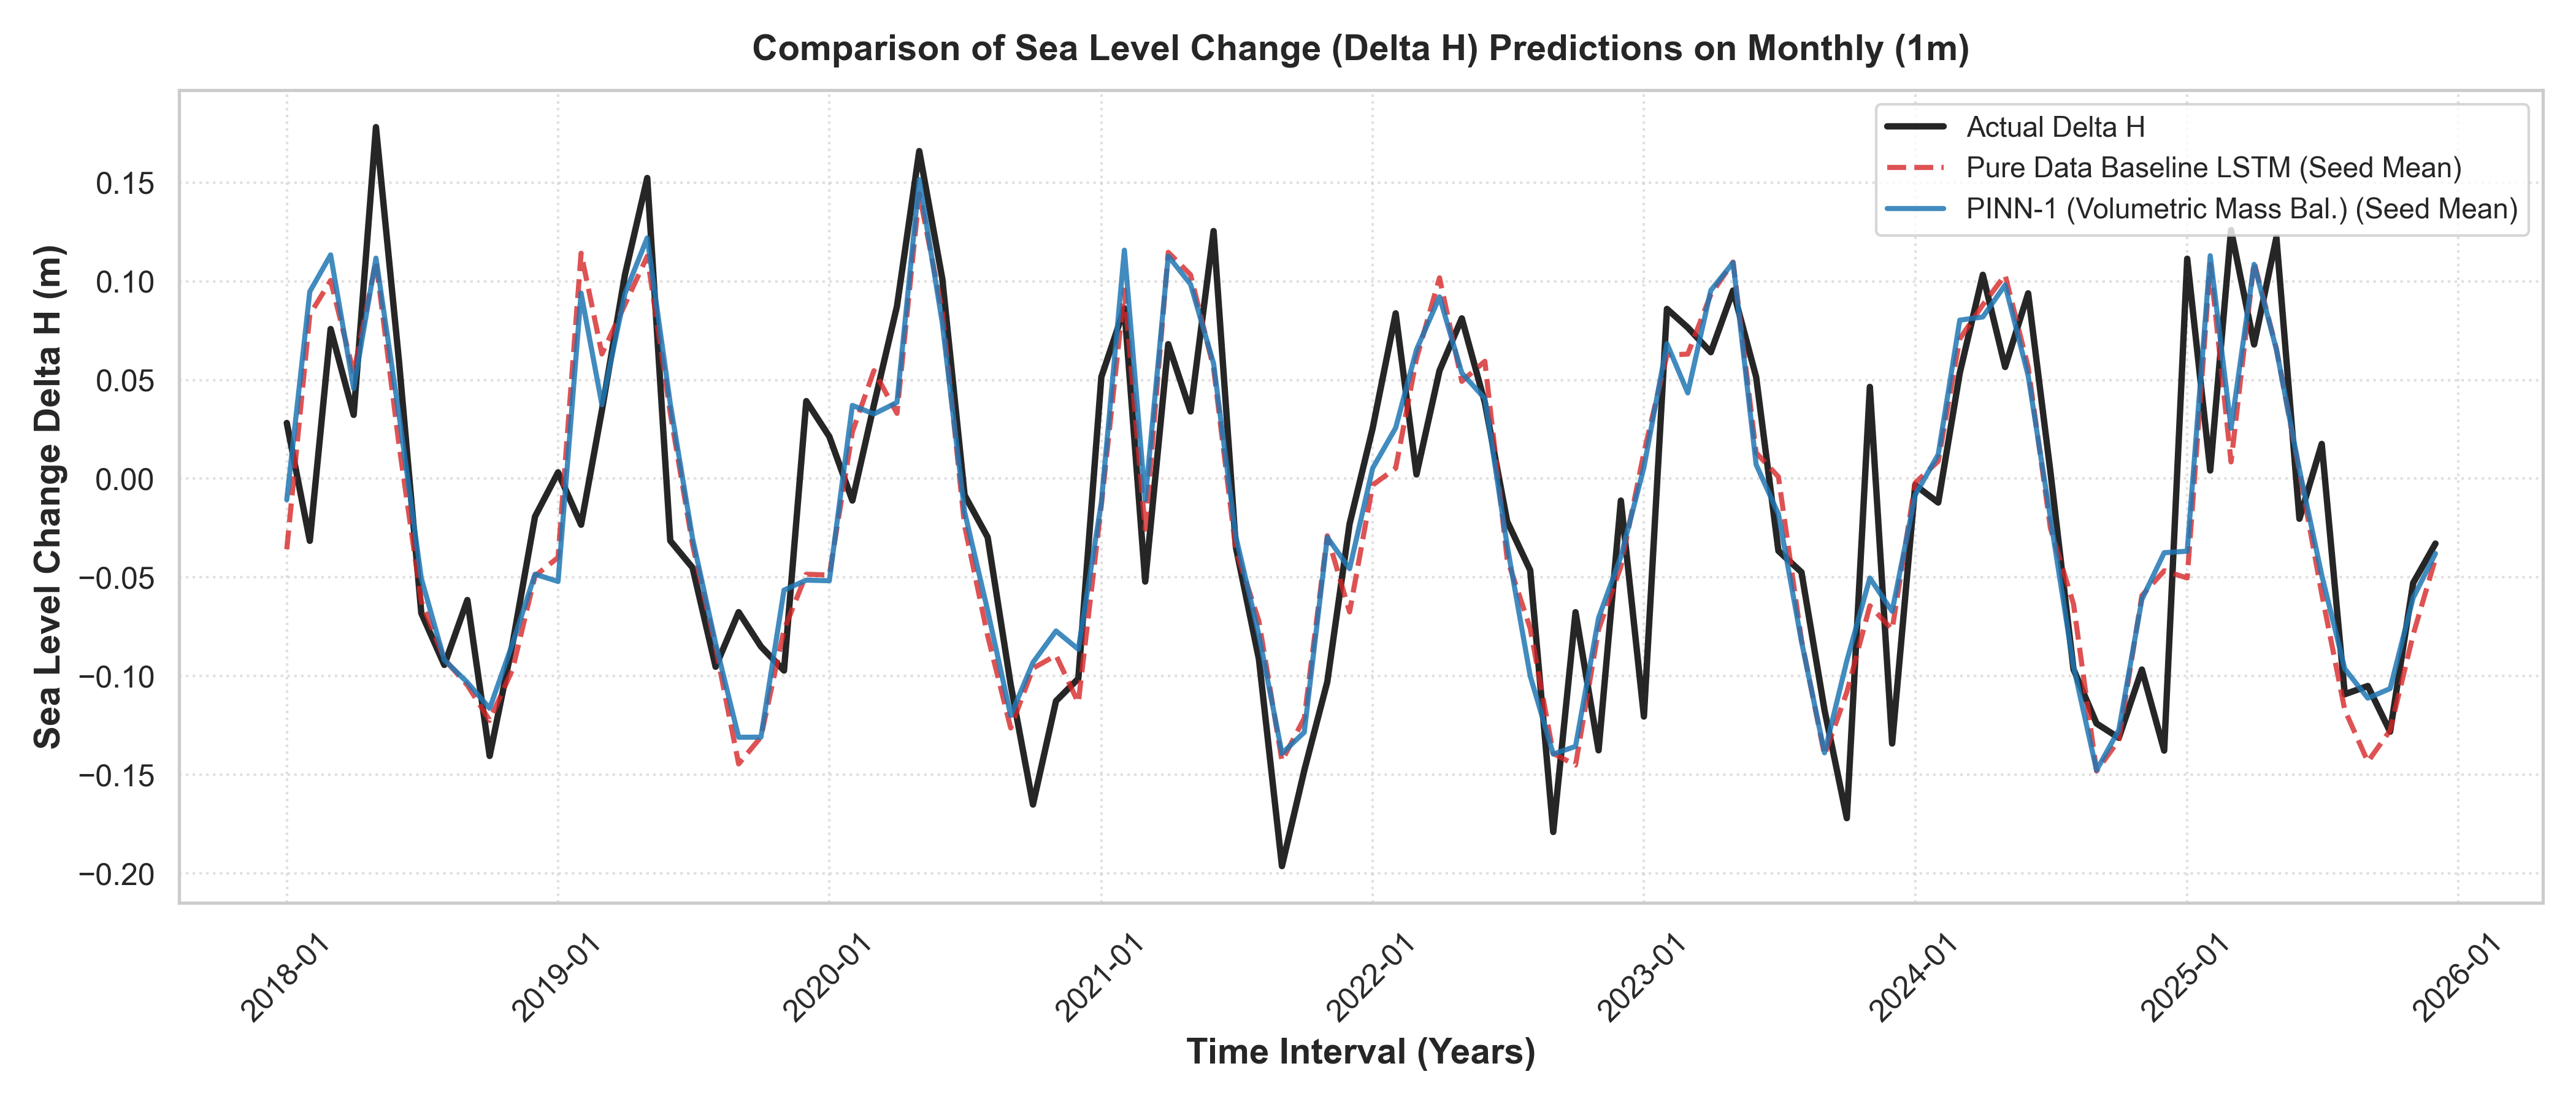
\includegraphics[width=\columnwidth]{../../figures/review_figures/fig4_1_monthly_predictions.png}
    \caption{PINN-3 test-set reconstruction (2018--2026).}
    \label{fig:pinn3_monthly}
\end{figure}

\subsection{$\lambda_{\text{phys}}$ Sensitivity}

PINN-1 optimally performs at $\lambda_{\text{phys}}{=}1.0$ (Table~\ref{tab:lambda}). Retraining at this value improved $R^2$ from $0.5252{\pm}0.0205$ to $0.6268{\pm}0.0230$ ($+19\%$).

\begin{table}[htbp]
\centering
\caption{PINN-1 $\lambda_{\text{phys}}$ sensitivity (single-seed).}
\label{tab:lambda}
\begin{tabular}{lccc}
\toprule
$\lambda_{\text{phys}}$ & \textbf{RMSE (m)} & \textbf{Corr.} & \textbf{$R^2$} \\
\midrule
0.1 & 0.0573 & 0.7856 & 0.5751 \\
0.5 & 0.0561 & 0.7893 & 0.5920 \\
1.0 & \textbf{0.0541} & \textbf{0.8084} & \textbf{0.6211} \\
5.0 & 0.0553 & 0.7942 & 0.6036 \\
\bottomrule
\end{tabular}
\end{table}

\subsection{Walk-Forward and Ablation}

Walk-forward CV (Table~\ref{tab:wf}) confirms regime-shift difficulty. Ablation (Table~\ref{tab:wf}) shows residual connection contributes modestly ($\Delta R^2{=}{+}0.0203$) and dynamic lake area improves $R^2$ to 0.5733. The Hybrid PINN achieves the highest single-run $R^2$ (0.6491). Thermodynamic walk-forward (Appendix) shows the Hybrid model consistently leads ($R^2{=}0.5791{\pm}0.0270$ vs.~PINN-2: $0.5378{\pm}0.0222$, PINN-3: $0.5222{\pm}0.0102$).

\begin{table}[htbp]
\centering
\caption{Walk-forward CV (baseline) and ablation (PINN-1 base).}
\label{tab:wf}
\begin{tabular}{lccc}
\toprule
\textbf{Experiment} & \textbf{RMSE (m)} & \textbf{$R^2$} \\
\midrule
Fold1\_2010 & 0.0700 & 0.3728 \\
Fold2\_2015 & 0.0597 & 0.5731 \\
Fold3\_2020 & 0.0659 & 0.4512 \\
\midrule
PINN-1 (base)         & 0.0605 & 0.5252 \\
No residual           & 0.0618 & 0.5049 \\
Dynamic area          & 0.0574 & 0.5733 \\
Hybrid (single-seed)  & 0.0520 & 0.6491 \\
\bottomrule
\end{tabular}
\end{table}

\subsection{Comprehensive Ranking}

Table~\ref{tab:ranking} consolidates all monthly $\Delta H$ results. The Hybrid PINN is excluded from the main ranking (single-seed only). Retrained models use optimized hyperparameters ($\lambda_{\text{phys}}{=}1.0$ for PINN-1; 600 epochs for PINN-2).

\begin{table}[htbp]
\centering
\caption{Consolidated monthly ranking (multi-seed, $n{=}5$).}
\label{tab:ranking}
\begin{tabular}{llcc}
\toprule
\textbf{Rank} & \textbf{Model} & \textbf{RMSE (m)} & \textbf{$R^2$} \\
\midrule
1 & PINN-3             & $0.0486{\pm}0.0003$ & $0.6939{\pm}0.0032$ \\
2 & PINN-2 (retrained) & $0.0521{\pm}0.0029$ & $0.6470{\pm}0.0396$ \\
3 & PINN-1 (retrained) & $0.0536{\pm}0.0017$ & $0.6268{\pm}0.0230$ \\
4 & PINN-2 River (retr.)& $0.0543{\pm}0.0023$ & $0.6174{\pm}0.0328$ \\
5 & Baseline           & $0.0568{\pm}0.0038$ & $0.5803{\pm}0.0556$ \\
6 & PINN-2 (original)  & $0.0572{\pm}0.0018$ & $0.5756{\pm}0.0259$ \\
7 & PINN-1 (original)  & $0.0605{\pm}0.0013$ & $0.5252{\pm}0.0205$ \\
\bottomrule
\end{tabular}
\end{table}

\begin{figure}[htbp]
    \centering
    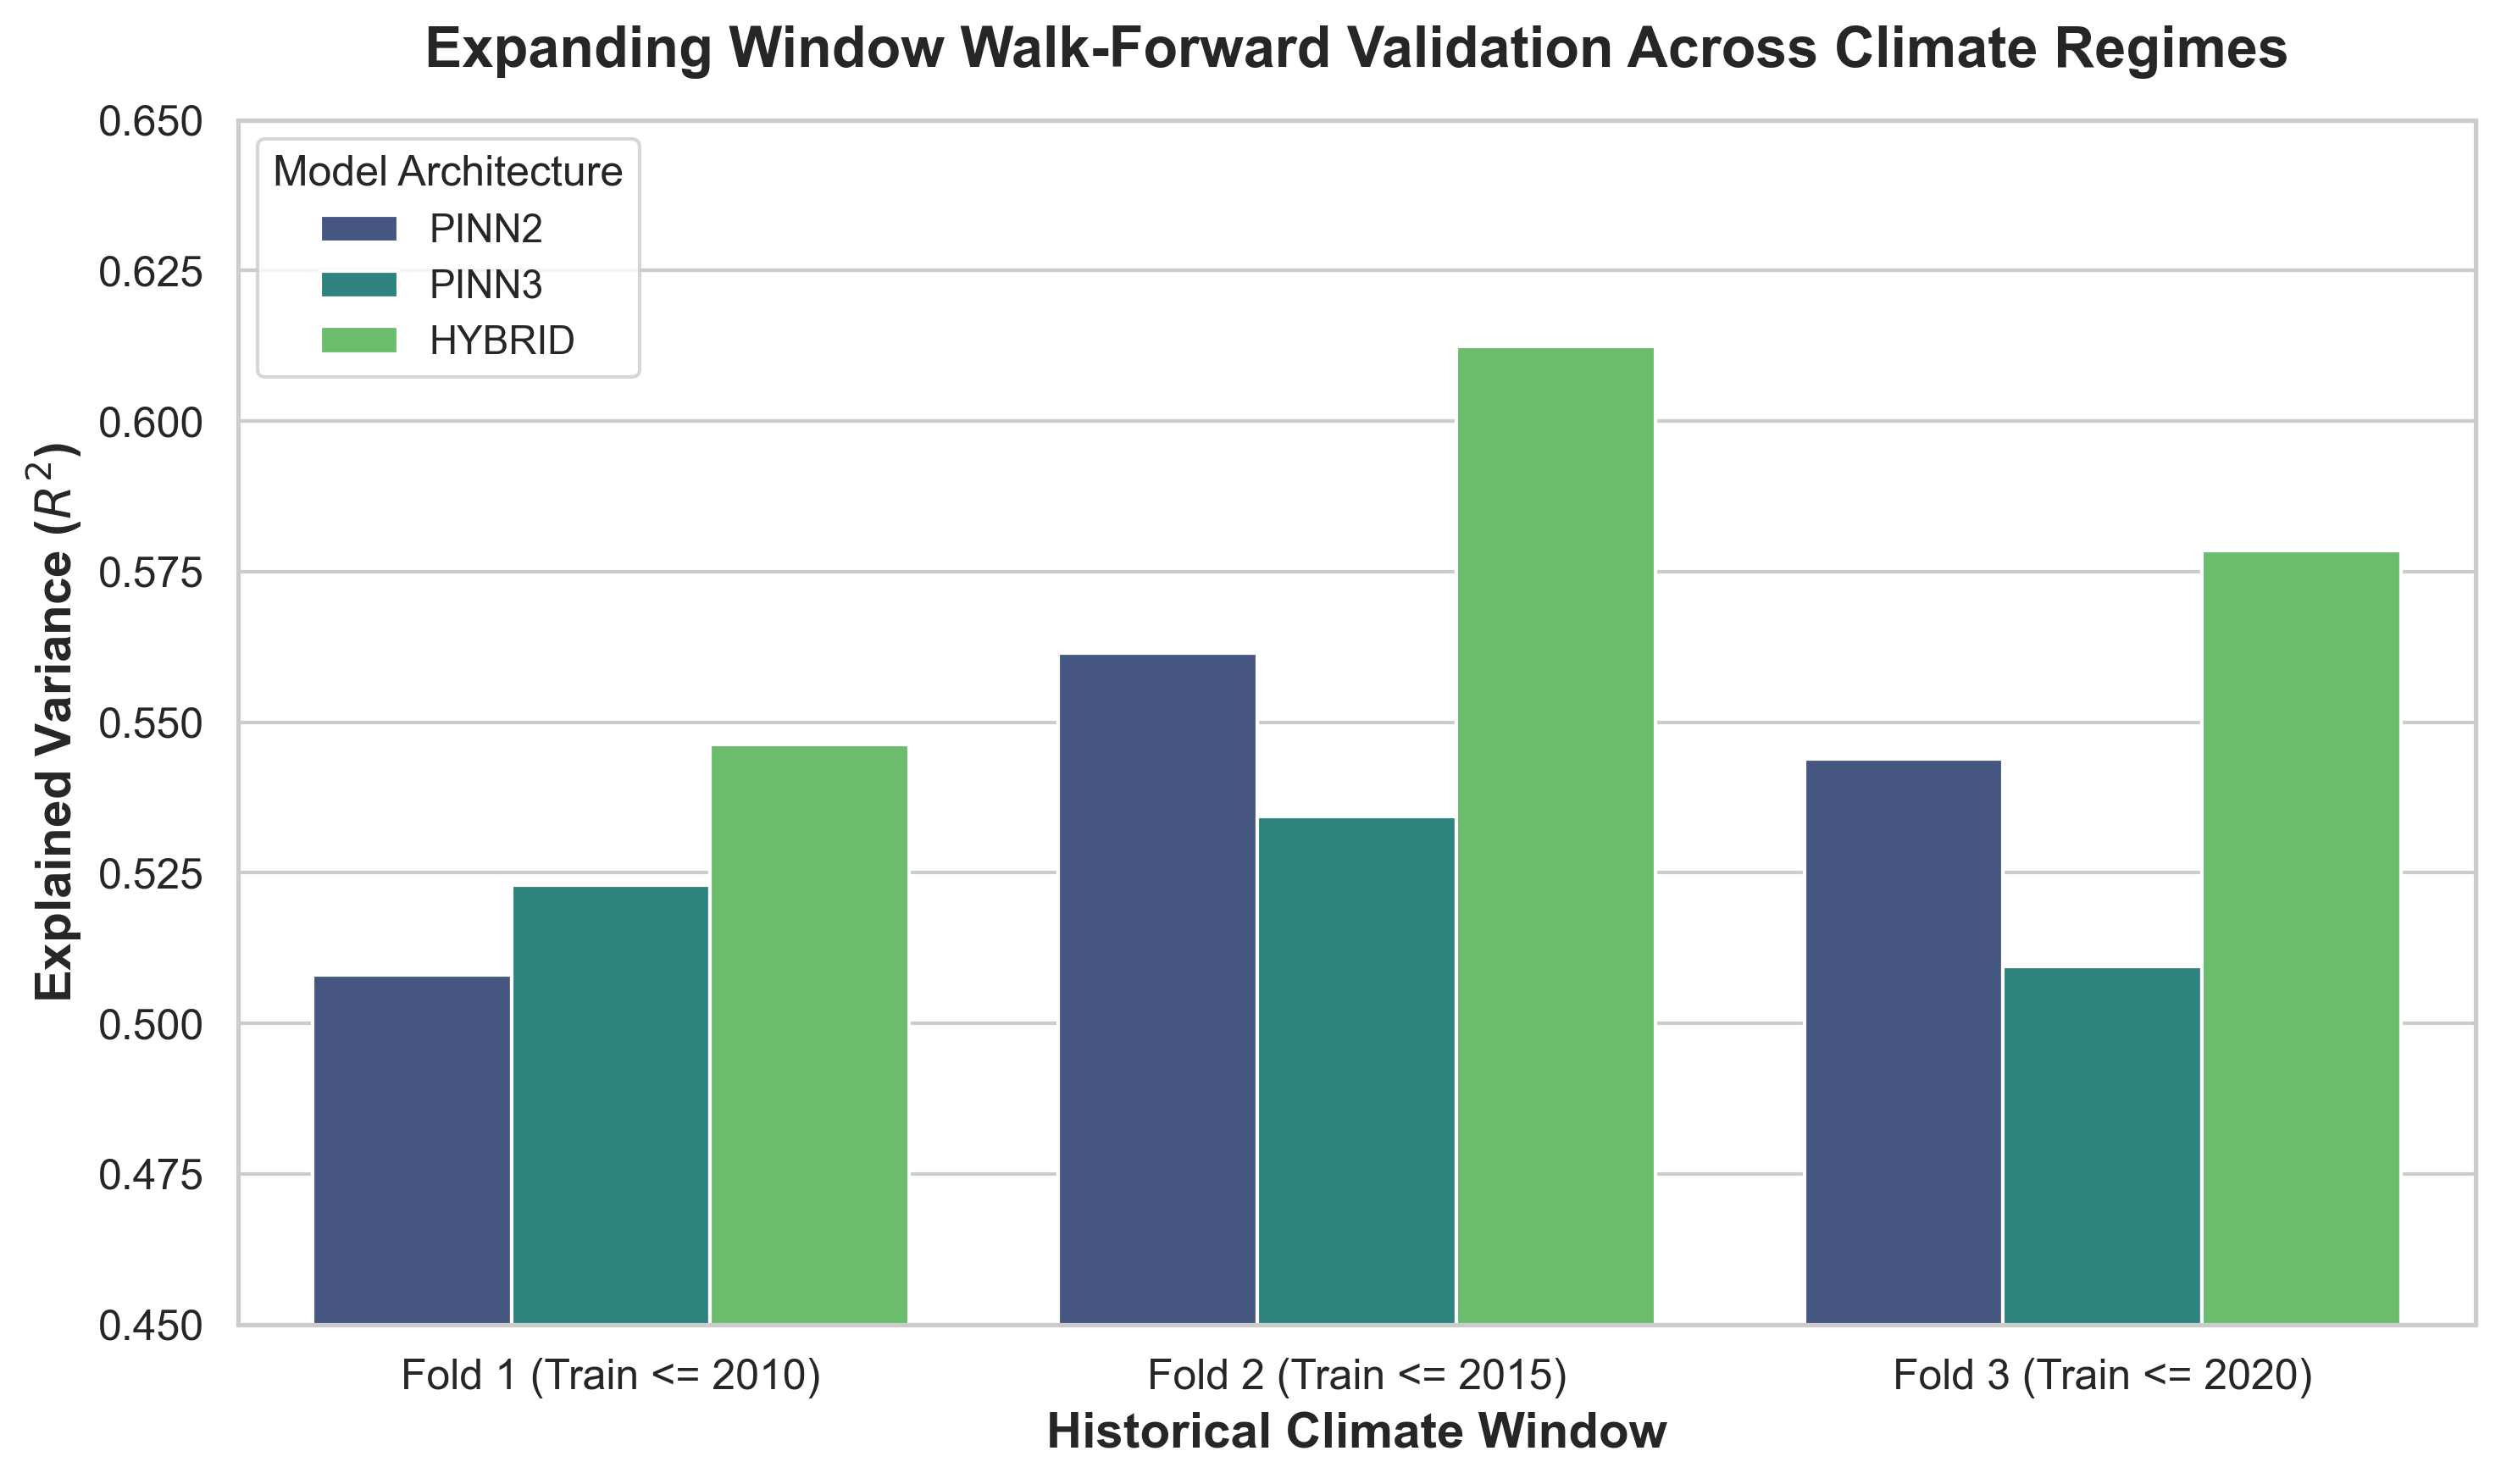
\includegraphics[width=\columnwidth]{../../figures/fig4_3_walk_forward_r2.png}
    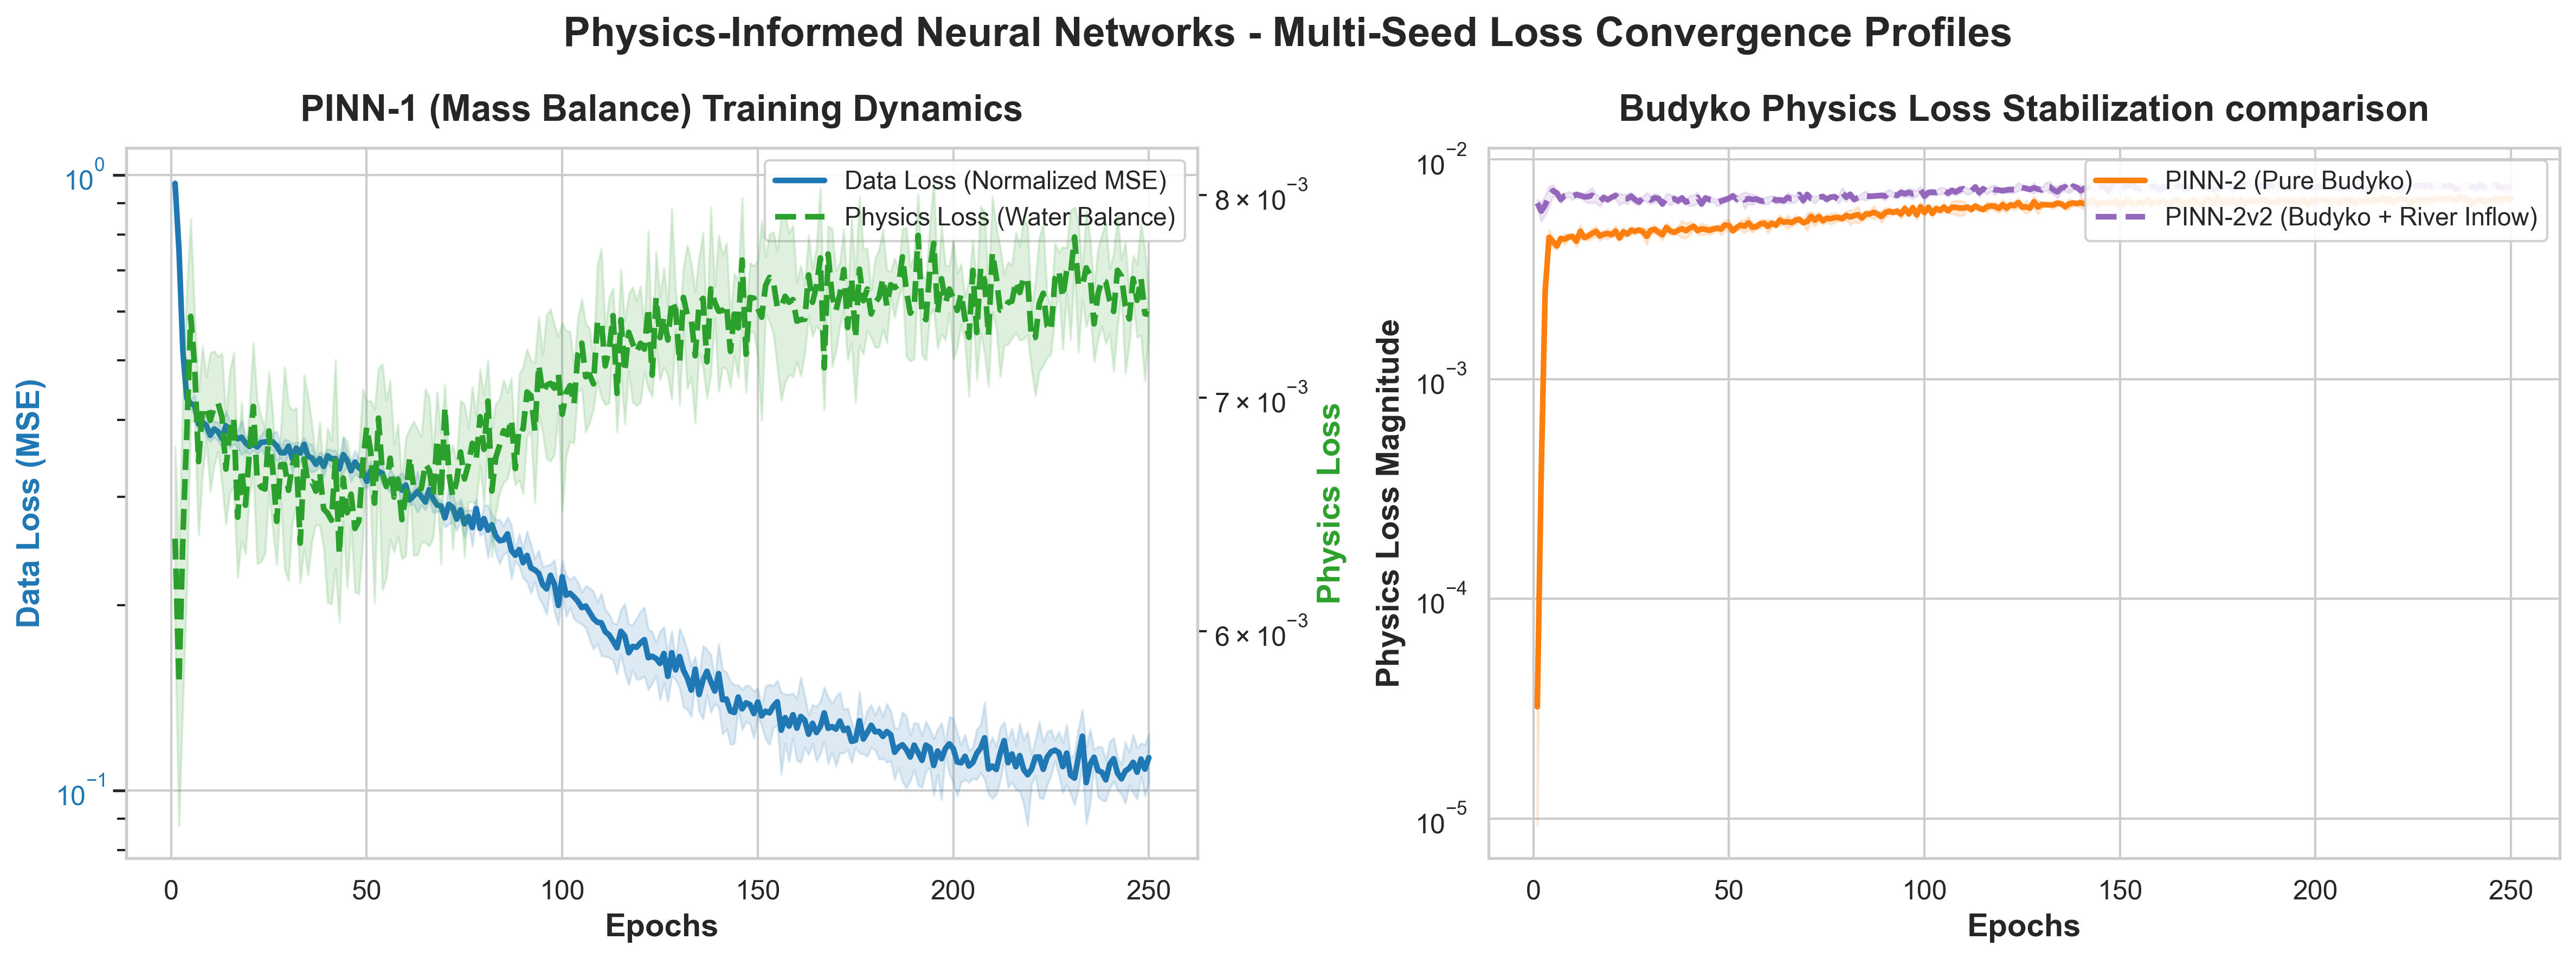
\includegraphics[width=\columnwidth]{../../figures/fig4_6_loss_curves_convergence.png}
    \caption{Walk-forward $R^2$ (left) and training loss curves (right).}
    \label{fig:supplementary}
\end{figure}

\section{Discussion}

\subsection{Physics Constraints: Skill vs. Stability}

The multi-seed results reveal a nuanced role for physics constraints~\eqref{eq:pinn1}--\eqref{eq:pinn3_evap}. The unconstrained baseline achieves competitive $R^2$ (0.5803) but with high seed sensitivity ($\pm0.0556$). Diebold-Mariano tests~\cite{diebold1995comparing} confirm this variability is statistically significant across seed pairs. Physics constraints provide three benefits: (1) PINN-3 achieves the highest $R^2$ (0.6939) with near-zero sensitivity ($\pm0.0032$); (2) all PINNs reduce initialization variance by 2--17$\times$; (3) at 10-day resolution, only physics-informed models achieve positive $R^2$, providing a structural prior against overfitting~\cite{huang2025physics,cuomo2022pinn}.

The finding that PINN-3 dominates on both predictive skill and stability suggests that evaporation, not runoff, is the dominant source of uncertainty in Caspian Sea level change at monthly scale. This aligns with prior evaporation-dominated budget analyses for the basin~\cite{samant2023climate}. Future work could test whether PINN-3's advantage generalizes to other closed basins or depends on Caspian-specific climate dynamics.

\subsection{Why Budyko Underperforms}

PINN-2's modest performance ($R^2{=}0.5756$) likely reflects the Budyko framework's annual-scale origins~\cite{cheng2025global}. At monthly resolution, seasonal storage dynamics confound the aridity-runoff relationship---water stored as snow or soil moisture during one month may become runoff months later, breaking the instantaneous $ET{=}f(P,PET)$ assumption. However, retraining substantially improves PINN-2 ($R^2{=}0.6470$), and the time-varying $n_t$ parameter~\cite{liu2025timevarying} partially compensates. The learned homoscedastic weighting further mitigates physics-data mismatch by automatically down-weighting the Budyko penalty when it conflicts with observations~\cite{kendall2017uncertainty}.

\subsection{Hybrid and Ablation Insights}

The Hybrid model demonstrates constraint complementarity, but its single-seed $R^2$ (0.6491) remains below multi-seed PINN-3 (0.6939), suggesting additional parameters increase optimization difficulty. The ablation study (Table~\ref{tab:wf}) reveals that dynamic lake area contributes meaningfully ($\Delta R^2{=}{+}0.0481$), while residual connections provide only a minor boost ($\Delta R^2{=}{+}0.0203$). All simple baselines (persistence, climatology) perform substantially worse, confirming neural models add value beyond naive forecasting.

\subsection{Activation Function Confound}
\label{sec:limitations}

The baseline and PINN-1 use ReLU activation while PINN-2 and PINN-3 use SiLU. This difference is a potential confound: SiLU's smooth, self-gating behavior could independently improve optimization, partially driving PINN-3's superior performance. While the shared backbone (layer count, dimensions, connectivity) isolates the first-order structural effect, the activation gap should be acknowledged. A SiLU-trained baseline and ReLU-trained PINN-3 would be needed to fully disentangle architecture from physics, but computational constraints precluded these additional experiments.

\subsection{Limitations}
Several limitations should be noted. The constant lake-area assumption introduces scaling uncertainty during the strong decline; a bathymetric curve is needed~\cite{samant2023climate}. PINN-2 served dual roles (screening and reference). The Hybrid PINN and ablation experiments are single-seed; multi-seed evaluation would strengthen conclusions. PINN-3 per-seed predictions were not stored in CSV format, preventing formal DM testing against the baseline. MC dropout uncertainty calibration (PICP) was not quantified. The dataset (396 monthly steps) and model size (${\sim}339$K parameters) yield approximately 1.15 samples per thousand parameters---warranting continued overfitting vigilance, though loss curves (Fig.~\ref{fig:supplementary}) and early stopping provide mitigation.

\subsection{Practical Recommendations}
For operational forecasting: PINN-3 is recommended for stability and pattern accuracy ($R^2{=}0.6939{\pm}0.0032$). The baseline may suffice for point predictions but is unreliable from single seeds. At 10-day and finer scales, physics-informed models are essential. The $\lambda_{\text{phys}}$ sensitivity analysis (Table~\ref{tab:lambda}) shows that even factors of 2--5$\times$ from optimal $\lambda$ preserve most of the physics benefit, making these models robust to imperfect calibration~\cite{raissi2019physics}.

\section{Conclusion}

This study provides the first systematic comparison of physics-informed neural networks for the Caspian Sea. Across 60 models, PINN-3 (Priestley--Taylor energy balance) achieves $R^2{=}0.6939{\pm}0.0032$---a 19.6\% improvement over the unconstrained baseline---with 2--17$\times$ lower seed sensitivity. Simple baselines (persistence $R^2{=}0.017$, climatology $R^2{=}0.0$) confirm the necessity of learned approaches.

Three practical findings emerge for the ML-for-science community: \textit{(1)} multi-seed evaluation is not optional---single-seed baseline $R^2$ varies by $\pm0.0556$, enough to incorrectly rank models; \textit{(2)} not all physics constraints improve skill---Budyko underperforms at monthly scale despite being the most theoretically grounded, while Priestley--Taylor excels; and \textit{(3)} the right physics constraint provides both accuracy and stability, but only when matched to the dominant process (here, evaporation over runoff).

For Caspian Sea forecasting, PINN-3 is recommended. The reproducible pipeline, public dataset~\cite{hersbach2020era5,munoz2021eraland,rodell2004gldas,schwatke2015dahiti,grimaldi2022glofas}, and open-source code at \url{https://github.com/fulaura/Caspian-Sea-level-prediction-PINN} provide a foundation for extending physics-aware modeling to other
closed-basin hydrological systems.

\section*{Appendix: Supplementary Results}

\subsection{10-Day Resolution}

Table~\ref{tab:10day} summarizes the multi-seed results at 10-day resolution.

\begin{table}[htbp]
\centering
\caption{10-day multi-seed (mean $\pm$ std, $n{=}5$).}
\label{tab:10day}
\begin{tabular}{lcc}
\toprule
\textbf{Model} & \textbf{RMSE (m)} & \textbf{$R^2$} \\
\midrule
Baseline & $0.0547{\pm}0.0013$ & $-0.1722{\pm}0.0555$ \\
PINN-1   & $0.0484{\pm}0.0008$ & $\phantom{-}0.0827{\pm}0.0302$ \\
PINN-2   & $0.0478{\pm}0.0006$ & $\phantom{-}0.1025{\pm}0.0241$ \\
PINN-3   & $0.0472{\pm}0.0011$ & $\phantom{-}0.0721{\pm}0.0410$ \\
\bottomrule
\end{tabular}
\end{table}

\subsection{Thermodynamic Walk-Forward}

Table~\ref{tab:thermo_walkforward} reports the thermodynamic walk-forward results across the three folds.

\begin{table}[htbp]
\centering
\caption{Thermodynamic walk-forward (best per fold in bold).}
\label{tab:thermo_walkforward}
\footnotesize
\begin{tabular}{llcc}
\toprule
\textbf{Fold} & \textbf{Model} & \textbf{RMSE (m)} & \textbf{$R^2$} \\
\midrule
Fold1\_2010 & Hybrid & \textbf{0.0596} & \textbf{0.5463} \\
            & PINN-3 & 0.0611 & 0.5229 \\
            & PINN-2 & 0.0620 & 0.5081 \\
Fold2\_2015 & Hybrid & \textbf{0.0569} & \textbf{0.6124} \\
            & PINN-2 & 0.0606 & 0.5614 \\
            & PINN-3 & 0.0624 & 0.5344 \\
Fold3\_2020 & Hybrid & \textbf{0.0578} & \textbf{0.5785} \\
            & PINN-2 & 0.0601 & 0.5438 \\
            & PINN-3 & 0.0623 & 0.5094 \\
\bottomrule
\end{tabular}
\end{table}

\subsection{PINN-2 River and Hybrid Architectures}

\textbf{PINN-2 River:} Treats Volga discharge as explicit inflow with Budyko for ungauged basin:
\begin{equation}
\Delta h_{\text{phys}} = (P_{\text{lake}} - E_{\text{lake}}) + \beta_{\text{volga}}\frac{Q_{\text{volga}}\Delta t}{A_{\text{lake}}} + (P_{\text{basin}} - ET_{\text{budyko}}) \cdot \text{scale}_t
\end{equation}

\textbf{Hybrid PINN:} Combines all three constraints. Outputs $\Delta h_{\text{pred}}$ plus all physics parameters ($\alpha_E,\beta_{\text{volga}},\gamma_{\text{other}},n_t,\text{scale}_t,\alpha_{\text{PT},t},C_{\text{wind},t},\gamma_{\text{runoff},t}$). Physics loss is unweighted sum of individual constraint losses, $\lambda_{\text{phys}}{=}1.0$.

\subsection{MC Dropout}

MC dropout (retrained PINN-1, 100 passes) achieved RMSE~=~0.0552~m, $R^2{=}0.6053$. Uncertainty bands widen during rapid level changes, indicating qualitative calibration.

\subsection{Data and Code Availability}

ERA5, ERA5-Land, GLDAS, DAHITI, and GloFAS data are publicly available~\cite{hersbach2020era5,munoz2021eraland,rodell2004gldas,schwatke2015dahiti,grimaldi2022glofas}. Code and trained models are available at \url{https://github.com/fulaura/Caspian-Sea-level-prediction-PINN}
\section*{Acknowledgment}
The first three authors thank Dr. A. Rakhimzhanova for supervision and guidance throughout this research.
\balance
\bibliographystyle{IEEEtran}
\bibliography{references}

\end{document}
